%%%%%%%% ICML 2025 EXAMPLE LATEX SUBMISSION FILE %%%%%%%%%%%%%%%%%
% Russian version of report.tex (same structure). Build: latexmk -pdf report_ru.tex

\documentclass{article}

% Recommended, but optional, packages for figures and better typesetting:
\usepackage{microtype}
\usepackage{graphicx}
\usepackage{subfigure}
\usepackage{booktabs} % for professional tables

% hyperref makes hyperlinks in the resulting PDF.
% If your build breaks (sometimes temporarily if a hyperlink spans a page)
% please comment out the following usepackage line and replace
% \usepackage{icml2025} with \usepackage[nohyperref]{icml2025} above.
\usepackage{hyperref}


% Attempt to make hyperref and algorithmic work together better:
\newcommand{\theHalgorithm}{\arabic{algorithm}}

% Use the following line for the initial blind version submitted for review:
% \usepackage{icml2025}

% If accepted, instead use the following line for the camera-ready submission:
\usepackage[accepted]{icml2025}

% Cyrillic: T2A encoding, Times-like Tempora with Cyrillic glyphs, decimal comma in math.
\usepackage[T2A]{fontenc}
\usepackage[utf8]{inputenc}
\usepackage[english,russian]{babel}
\usepackage{tempora}
\usepackage{icomma}

% icml2025.sty and algorithm.sty hard-code English labels; replace them.
\makeatletter
\renewcommand{\Notice@String}{Отчёт по тестовому заданию: воспроизведение ALDA \citep{batra2024alda}, октябрь 2026.}
\def\fnum@figure{Рис.~\thefigure}
\def\fnum@table{Таблица~\thetable}
\renewcommand{\ALG@name}{Алгоритм}
\renewenvironment{abstract}
   {\centerline{\large\bf Аннотация}\vspace{-0.12in}\begin{quote}}
   {\par\end{quote}\vskip 0.12in}
\renewcommand{\printAffiliationsAndNotice}[1]{%
\stepcounter{@affiliationcounter}%
{\let\thefootnote\relax\footnotetext{\hspace*{-\footnotesep}\ifdefined\isaccepted #1\fi%
\forloop{@affilnum}{1}{\value{@affilnum} < \value{@affiliationcounter}}{
\textsuperscript{\arabic{@affilnum}}\csname @affilname\the@affilnum\endcsname}.
Связь с автором: \icmlcorrespondingauthor@text.

\ \\
\Notice@String
}
}
}
\makeatother

% For theorems and such
\usepackage{amsmath}
\usepackage{amssymb}
\usepackage{mathtools}
\usepackage{amsthm}

%%%%%%%%%%%%%%%%%%%%%%%%%%%%%%%%
% THEOREMS
%%%%%%%%%%%%%%%%%%%%%%%%%%%%%%%%
\theoremstyle{plain}
\newtheorem{theorem}{Теорема}[section]
\newtheorem{proposition}[theorem]{Утверждение}
\newtheorem{lemma}[theorem]{Лемма}
\newtheorem{corollary}[theorem]{Следствие}
\theoremstyle{definition}
\newtheorem{definition}[theorem]{Определение}
\newtheorem{assumption}[theorem]{Предположение}
\theoremstyle{remark}
\newtheorem{remark}[theorem]{Замечание}


% The \icmltitle you define below is probably too long as a header.
% Therefore, a short form for the running title is supplied here:
\icmltitlerunning{\smash{Воспроизведение ALDA: zero-shot обобщение без аугментации данных}}

\begin{document}

\twocolumn[
\icmltitle{Воспроизведение ALDA: zero-shot обобщение в визуальном RL \\
           без аугментации данных}

\begin{icmlauthorlist}
\icmlauthor{Олег Жуков}{ind}
\end{icmlauthorlist}

\icmlaffiliation{ind}{Независимый исследователь}

\icmlcorrespondingauthor{Олег Жуков}{zhukovol3q@gmail.com}

\icmlkeywords{обучение с подкреплением, распутанные представления, ассоциативная память, обобщение}

\vskip 0.3in
]

\printAffiliationsAndNotice{}

\begin{abstract}
Мы заново реализуем ALDA (Associative Latent DisentAnglement). Метод
добавляет к Soft Actor-Critic распутанное латентное пространство в стиле
QLAE, в котором покомпонентные кодовые книги работают как ассоциативная
память. Мы проверяем, обобщается ли такой агент на визуальные сдвиги
распределения без дообучения и без какой-либо аугментации данных. Агент
обучается на задаче \emph{walker-walk} из DeepMind Control по пикселям в
течение 1~млн шагов среды (2 сида); периодически мы оцениваем его в среде со
сдвигом цвета и в Distracting Control Suite (уровень easy: динамические фоны
DAVIS, возмущения камеры и цвета). На обучающей среде агент набирает
награду~778, при сдвиге цвета сохраняет 81\% от неё, в Distracting CS~---
43\%, причём обе кривые на OOD-средах продолжают расти к концу обучения.
Реконструкции показывают, что латентная модель переводит кадры с помехами
обратно к виду обучающей среды. Однако величина этой ассоциативной поправки
не предсказывает разрыв в награде между отдельными оценками.
\end{abstract}

\section{Введение}
\label{sec:intro}

Стратегии, обученные по пикселям, обычно перестают работать, когда меняется
внешний вид сцены. Стандартное решение~--- аугментация данных
\citep{yarats2021drqv2,hansen2021svea}: во время обучения агенту показывают
приближения тех изменений, которые встретятся при тестировании. ALDA
\citep{batra2024alda} обходится без аугментации. Метод обучает распутанное
латентное представление с помощью квантования латентов \citep{hsu2023qlae} и
трактует квантованную латентную модель как ассоциативную память в духе сетей
Хопфилда: при тестировании кодировка вне обучающего распределения (OOD) в
каждой латентной размерности притягивается к ближайшему запомненному значению.
В идеале изменение фактора, не важного для задачи (например, фона), затрагивает
лишь несколько латентов, и они возвращаются к знакомым значениям.

В этом отчёте описана реализация SAC+ALDA с нуля в одном файле на основе SAC
из CleanRL \citep{huang2022cleanrl}. Агент обучается в DeepMind Control
\citep{tassa2018dmc} и проверяется на zero-shot перенос в Distracting Control
Suite \citep{stone2021dcs}. Мы ставим один исследовательский вопрос:
\emph{действительно ли ассоциативная латентная модель срабатывает на
OOD-наблюдениях и объясняет ли величина её поправки падение качества?}
(раздел~\ref{sec:rq}).

\section{Метод}
\label{sec:method}

\paragraph{SAC.} Базовый алгоритм~--- Soft Actor-Critic
\citep{haarnoja2018sac}: стратегия в виде гауссианы, пропущенной через tanh,
два критика с целевыми сетями, обновляемыми усреднением Поляка, и
автоматическая настройка температуры энтропии.

\paragraph{Распутывание (QLAE).} Энкодер $f_\theta$ переводит \emph{один}
RGB-кадр в непрерывный вектор $z_{cont}\in\mathbb{R}^{n_z}$. У каждой
размерности $j$ своя скалярная кодовая книга $v_j\in\mathbb{R}^{|V|}$, а
декодер $g_\phi$ восстанавливает кадр по квантованному латенту. Распутыванию
способствуют сильное затухание весов $f_\theta$ и $g_\phi$ вместе с
покомпонентным квантованием \citep{hsu2023qlae}.

\paragraph{Ассоциация.} ALDA заменяет жёсткий $\arg\min$ из QLAE на
извлечение из современной сети Хопфилда \citep{ramsauer2020hopfield}
отдельно по каждой размерности:
\begin{equation}
  z_{d,j} = \textstyle\sum_k \mathrm{softmax}\big(-\beta\,|z_{cont,j}-v_{jk}|\big)_k\, v_{jk}.
  \label{eq:assoc}
\end{equation}
При большом $\beta$ это извлекает (почти) одно запомненное значение на
размерность. Кодовая книга \emph{не} подтягивается к выходам энкодера (нет
$\mathcal{L}_{quantize}$): её оптимизирует только функция потерь задачи
(критика), поэтому значения работают как память, настроенная под задачу, и
энкодер должен научиться попадать в неё. Целевая функция ALDA:
\begin{equation}
  \begin{aligned}
  \mathcal{L}_{ALDA} = {} & \|g_\phi(\tilde z) - o\|_2^2 + \|z_{cont} - \mathrm{sg}(z_d)\|_2^2 \\
  & + \lambda_\theta\|\theta\|^2 + \lambda_\phi\|\phi\|^2,
  \end{aligned}
\end{equation}
где $\tilde z = z_{cont} + \mathrm{sg}(z_d - z_{cont})$~--- straight-through
оценка градиента, $\mathrm{sg}$~--- остановка градиента. Второе слагаемое
называется потерей привязки (commitment).

\paragraph{Временная информация.} Стек из $k{=}3$ кадров сворачивается в
размерность батча: каждый кадр кодируется и проходит ассоциацию независимо,
после чего $k$ латентных векторов объединяет по времени небольшая одномерная
свёрточная сеть $h_\gamma$ (алгоритм~\ref{alg:alda}). Так автокодировщик всегда
работает с отдельными изображениями; авторы статьи показали, что это
необходимо для распутывания.

\begin{algorithm}[tb]
   \caption{Обновление SAC+ALDA (один шаг градиента)}
   \label{alg:alda}
\begin{algorithmic}
   \STATE {\bfseries Вход:} батч $(o, a, r, o', d)$, $o\in\mathbb{R}^{B\times 3k\times64\times64}$
   \STATE $x \leftarrow$ $o$, разложенный на $Bk$ отдельных кадров
   \STATE $z_{cont} \leftarrow f_\theta(x)$; \ $z_d \leftarrow l_\psi(\mathrm{sg}(z_{cont}))$ \hfill (\ref{eq:assoc})
   \STATE $\mathcal{L}_{ALDA} \leftarrow \mathrm{MSE}(g_\phi(z_{cont}{+}\mathrm{sg}(z_d{-}z_{cont})), x) + \mathrm{MSE}(z_{cont}, \mathrm{sg}(z_d))$
   \STATE $h \leftarrow h_\gamma(z_d$, приведённый к форме $B\times k\times n_z)$
   \STATE $y \leftarrow r + \gamma(1{-}d)\big(\min_i \bar Q_i(h', a') - \alpha\log\pi(a'|h')\big)$, $a'\sim\pi(\cdot|h')$
   \STATE $\mathcal{L}_Q \leftarrow \sum_i (Q_i(h,a) - y)^2$
   \STATE шаг AdamW по $(\theta,\phi,\psi,\gamma,Q)$ для $\mathcal{L}_Q + \mathcal{L}_{ALDA}$
   \STATE \textbf{на каждом втором шаге:} обновить $\pi$ и $\alpha$ по $\mathrm{sg}(h)$; обновить $\bar Q, \bar h_\gamma$ усреднением Поляка
\end{algorithmic}
\end{algorithm}

\section{Реализация}
\label{sec:impl}

Код~--- один файл (\texttt{alda.py}, около 570 строк) и конфигурации YAML;
все гиперпараметры взяты из таблицы в приложении статьи
(табл.~\ref{tab:hparams}).

\paragraph{Архитектура.} Энкодер и декодер повторяют приложение QLAE, только
leaky ReLU заменены на GELU, как в ALDA. \emph{Энкодер:} 4 блока [свёртка
$3{\times}3$ с шагом 1, свёртка $3{\times}3$ с шагом 1, свёртка $4{\times}4$ с
шагом 2] шириной 32/64/128/256 каналов; после каждой свёртки идут GELU и
InstanceNorm ($64^2\!\to\!4^2$), затем два полносвязных слоя по 256 нейронов с
ReLU и линейный слой в $n_z{=}12$. \emph{Декодер} устроен как в StyleGAN: $z$
проходит через двухслойную сеть и превращается в вектор стиля $w$; обучаемый
вход $256{\times}4{\times}4$ увеличивается двенадцатью слоями транспонированной
свёртки, выходы которых модулируются через AdaIN по $w$, а свёртка
$1{\times}1$ выдаёт RGB. \emph{Латентная модель:} скалярные кодовые книги
$12{\times}12$, инициализированные как $\mathrm{linspace}(-1,1)$, $\beta{=}100$.
\emph{Энкодер истории:} два слоя Conv1d (ядро 2, 64 канала, GELU) поверх
латентов трёх кадров. Критик проецирует их выход линейным слоем в
50~признаков, за которыми идут две Q-сети ($2{\times}1024$, GELU); у актора
своя 50-мерная проекция и сеть $2{\times}1024$ с tanh-гауссовой стратегией.

\paragraph{Маршрутизация градиентов.} Мы следуем своему прочтению рис.~2
статьи. $\mathcal{L}_Q$ обучает Q-сети, энкодер истории и значения кодовой
книги, но не проходит дальше $z_{cont}$: энкодер получает градиенты
\emph{только} от реконструкции и привязки. Актор использует выход энкодера
истории критика с остановкой градиента, как в SAC+AE \citep{yarats2021sacae}.

\paragraph{Отклонения от статьи и инженерные решения.}
\textbf{(i) Раздельное затухание весов.} С Adam и обычной L2-регуляризацией
$0,1$ градиент регуляризации подавлял градиент реконструкции, и в начале
обучения энкодер схлопывался в константу. Поэтому мы используем AdamW
\citep{loshchilov2019adamw}, как в реализации самих авторов QLAE, с затуханием
$0,1$ только для энкодера и декодера.
\textbf{(ii) Кодирование следующего наблюдения.} Кадры кодируются
независимо, поэтому $o'$ разделяет с $o$ $k{-}1$ кадров; мы переиспользуем их
латенты и для TD-цели кодируем только новый кадр. Результат тот же, а
вычислений примерно вдвое меньше.
\textbf{(iii) Эффективность.} Буфер воспроизведения хранит только последний
кадр каждого перехода и собирает стеки при выборке; энкодер и декодер
работают в смешанной точности bf16 (латентная модель, критик и актор
остаются в fp32); сцена рендерится один раз на шаг агента, а не на каждый
повтор действия.
\textbf{(iv) Ограничение эпизода по времени} не считается терминальным
состоянием, и целевое значение по-прежнему строится через бутстрэп.

\begin{table}[t]
\caption{Гиперпараметры (одинаковы для обоих сидов).}
\label{tab:hparams}
\vskip 0.1in
\begin{center}
\begin{small}
\begin{tabular}{lr}
\toprule
Параметр & Значение \\
\midrule
Ёмкость буфера / размер батча & $10^6$ / 128 \\
Температура ассоциации $\beta$ & 100 \\
Латентов $n_z$ / значений в книге $|V|$ & 12 / 12 \\
Затухание весов $\lambda_\theta{=}\lambda_\phi$ & $0,1$ \\
Стек кадров / повтор действия & 3 / 4 \\
Наблюдение & $9\times64\times64$ \\
Скорость обучения / для $\alpha$ & $10^{-3}$ / $10^{-4}$ \\
Начальная температура $\alpha$ & $0,1$ \\
Период обновл. актора / целевых & 2 / 2 \\
Коэффициент Поляка $\tau$ / дисконт $\gamma$ & $0,005$ / $0,99$ \\
Размерность признаков ($z_Q$, $z_\pi$) & 50 \\
Случайные действия в начале & 1000 шагов агента \\
\bottomrule
\end{tabular}
\end{small}
\end{center}
\vskip -0.1in
\end{table}

\section{Постановка экспериментов}
\label{sec:setup}

\paragraph{Обучение.} Агент обучается на \emph{walker-walk} по пикселям
$64{\times}64$ в течение $10^6$ шагов среды ($2,5{\cdot}10^5$ шагов агента,
одно обновление градиента на шаг агента), 2 сида. Каждый запуск занял около
9 часов на одной RTX~3090 вместе с оценкой. Аугментация не используется
нигде: агент видит только стандартную сцену DMC.

\paragraph{Zero-shot оценка.} Каждые $10^4$ шагов среды мы проводим 5
детерминированных эпизодов (tanh от среднего стратегии) в трёх средах с
сидами, не пересекающимися с обучающими:
\begin{itemize}
\item \textbf{Обучающая среда}: исходная задача DMC.
\item \textbf{Сдвиг цвета}: цветовое возмущение из DCS с
  $\texttt{max\_delta}{=}0,5$ без дрейфа. Цвета агента и пола сдвигаются на
  величину до $\pm0,5$ по каждому каналу RGB, один раз за эпизод. Это наша
  замена среды «color hard» из DMCGB, которую использовали авторы; идея
  похожая, но среды не совпадают.
\item \textbf{Distracting CS (easy)}: на фоне динамические видео из
  валидационной части DAVIS 2017 \citep{ponttuset2017davis} (4 видео), плюс
  динамические возмущения камеры и цвета с масштабом $0,1$ \citep{stone2021dcs}.
\end{itemize}
Кроме награды, при каждой оценке мы считаем латентные статистики по всем
кадрам оценочных эпизодов: средний ассоциативный сдвиг $|z_{cont}-z_d|$, долю
компонент $z_{cont}$ за пределами диапазона своей кодовой книги, нормированную
энтропию использования кодовой книги и MSE реконструкции относительно
наблюдаемого кадра.

\section{Результаты}
\label{sec:results}

\begin{figure}[t]
\vskip 0.1in
\begin{center}
\centerline{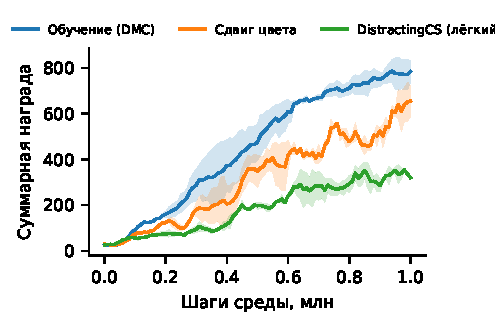
\includegraphics[width=\columnwidth]{figures/returns_ru}}
\caption{Награда при оценке на walker-walk в зависимости от числа шагов
среды. Линии~--- среднее по 2 сидам (скользящее среднее по 5 оценкам),
заливка~--- разброс между сидами. OOD-среды во время обучения не
встречаются.}
\label{fig:returns}
\end{center}
\vskip -0.2in
\end{figure}

\begin{table}[t]
\caption{Награда при оценке, усреднённая за последние $10^5$ шагов
(11 оценок $\times$ 5 эпизодов). «Доля»~--- отношение к награде на
обучающей среде.}
\label{tab:returns}
\vskip 0.1in
\begin{center}
\begin{small}
\begin{tabular}{lcccc}
\toprule
Среда & Сид 1 & Сид 2 & Среднее & Доля \\
\midrule
Обучающая      & 722 & 833 & 778 & $1,00$ \\
Сдвиг цвета    & 589 & 668 & 628 & $0,81$ \\
DistractingCS  & 329 & 339 & 334 & $0,43$ \\
\bottomrule
\end{tabular}
\end{small}
\end{center}
\vskip -0.1in
\end{table}

\paragraph{Кривые обучения.} Рис.~\ref{fig:returns} и табл.~\ref{tab:returns}
подводят итог. На обучающей среде оба сида достигают награды 700--850 к
1~млн шагов, и кривая всё ещё растёт. Zero-shot качество появляется в обеих
OOD-средах и растёт до конца обучения: при сдвиге цвета награда доходит
примерно до 630 (81\%), в Distracting CS~--- примерно до 330 (43\%), тогда как
случайно инициализированный агент получает около 30 во всех трёх средах.
Разброс в OOD-средах большой: стандартное отклонение по 5 эпизодам одной
оценки составляет 150--200 против 40--50 на обучающей среде. Часть эпизодов
переносится почти идеально, часть проваливается; это согласуется с тем, что
помехи выбираются заново в каждом эпизоде.

\begin{figure*}[t]
\vskip 0.1in
\begin{center}
\centerline{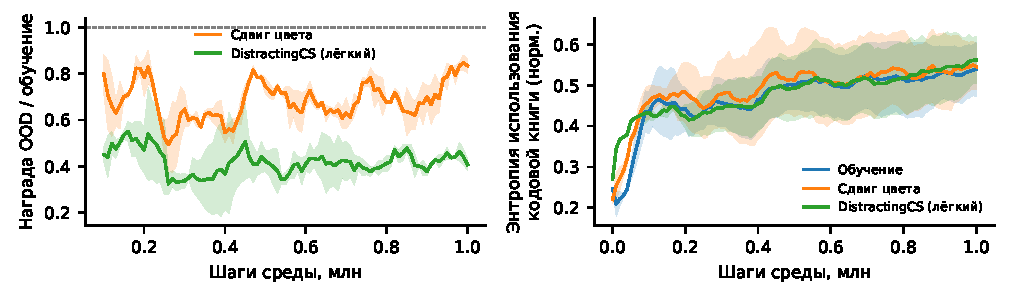
\includegraphics[width=\textwidth]{figures/retention_entropy_ru}}
\caption{Слева: награда в OOD-среде как доля награды на обучающей среде
(начиная с $10^5$ шагов, скользящее среднее по 5 оценкам; заливка~--- разброс
между сидами). Справа: нормированная энтропия использования кодовой книги на
оценочных кадрах из каждой среды.}
\label{fig:retention}
\end{center}
\vskip -0.2in
\end{figure*}

\paragraph{Доля сохранённой награды.} Если разделить награду в OOD-среде на
награду в обучающей (рис.~\ref{fig:retention}, слева), уходит эффект того,
что агент просто стал лучше решать саму задачу. В Distracting CS эта доля всё
обучение держится примерно на уровне $0,35$--$0,5$, так что абсолютный рост
награды в DCS на рис.~\ref{fig:returns} в основном отражает прогресс на
обучающей задаче. При сдвиге цвета доля проседает примерно до $0,6$ между
$0,3$ и $0,8$~млн шагов и восстанавливается примерно до $0,85$ к 1~млн.
Энтропия использования кодовой книги (рис.~\ref{fig:retention}, справа)
растёт первые $2{\cdot}10^5$ шагов, а затем медленно увеличивается. На
обучающих и OOD-кадрах она почти одинакова, то есть OOD-входы распределяются
по запомненным значениям так же широко, как обучающие.

\begin{figure}[t]
\vskip 0.1in
\begin{center}
\centerline{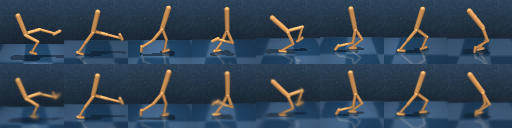
\includegraphics[width=\columnwidth]{figures/recon_train_s1}}
\vskip 0.03in
\centerline{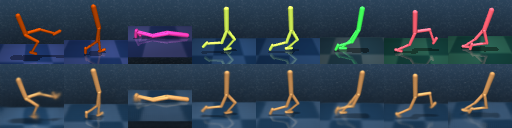
\includegraphics[width=\columnwidth]{figures/recon_color_s1}}
\vskip 0.03in
\centerline{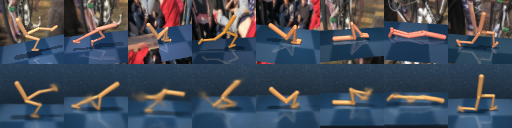
\includegraphics[width=\columnwidth]{figures/recon_dcs_s1}}
\caption{Входы (верхняя строка каждой пары) и реконструкции $g_\phi(z_d)$
(нижняя) после 1~млн шагов, сид 1. Сверху вниз: обучающая среда, сдвиг цвета,
Distracting CS. Цвета и фоны DAVIS из OOD-сред заменяются видом обучающей
среды (оранжевый агент, синий пол в клетку), поза в основном сохраняется.}
\label{fig:recon}
\end{center}
\vskip -0.2in
\end{figure}

\paragraph{Реконструкции.} На рис.~\ref{fig:recon} видна работа ассоциации.
При сдвиге цвета перекрашенный агент (красный, зелёный, пурпурный) и
тонированный пол декодируются как обычный оранжевый агент на синем полу,
с правильной позой. В Distracting CS фон DAVIS (люди, велосипеды) полностью
исчезает, и декодер рисует пол и небо из обучающей среды. Ошибки появляются в
позе. На нескольких реконструкциях из DCS конечности размыты или расположены
неверно, вероятно, потому, что возмущение камеры сдвигает агента в кадре, а
такого важного для задачи изменения в обучающих данных не было.

\begin{figure}[t]
\vskip 0.1in
\begin{center}
\centerline{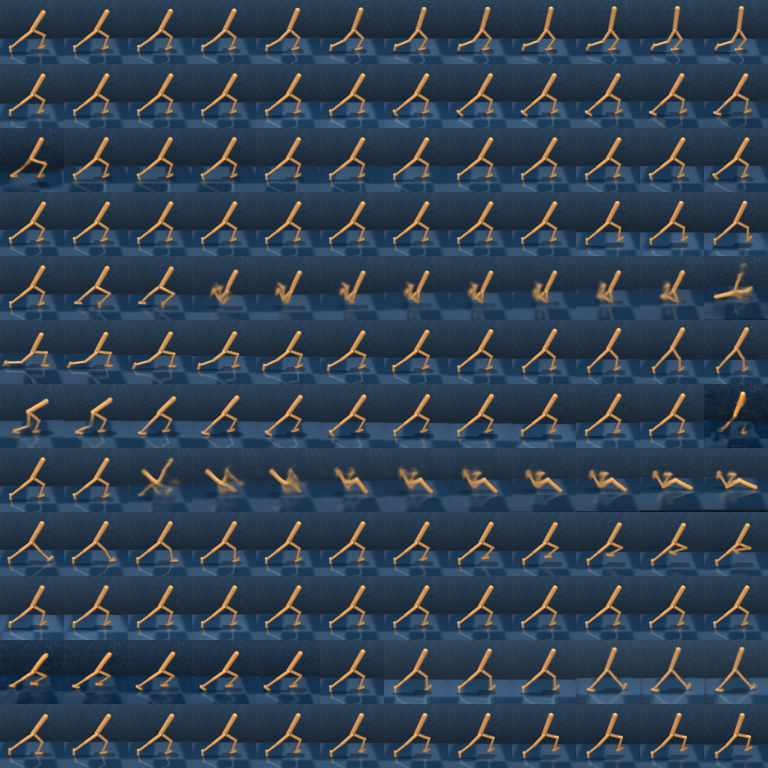
\includegraphics[width=0.9\columnwidth]{figures/traversal_s1}}
\caption{Обход латентных переменных после 1~млн шагов (сид 1). Строка $i$
перебирает 12 отсортированных значений кодовой книги латента $i$, остальные
латенты зафиксированы на $z_d$ обучающего кадра.}
\label{fig:traversal}
\end{center}
\vskip -0.2in
\end{figure}

\paragraph{Обход латентных переменных.} По рис.~\ref{fig:traversal} видно,
что отдельные латенты управляют понятными частями позы агента: одни строки
двигают одну ногу вперёд-назад, строки 5 и 8 переводят корпус из
вертикального положения в падение или лежачее, другие немного смещают тело по
высоте или горизонтали. Внешний вид обучающей сцены никогда не меняется,
поэтому ни один латент не кодирует фон или цвет. Это ожидаемо и означает, что
с OOD-внешним видом может справиться только ассоциация: отдельного латента,
который поглотил бы помеху, нет. Распутывание неидеально: латенты корпуса
заодно сгибают ноги. Энтропия использования кодовой книги в конце обучения
составляет $0,60$ и $0,47$ от максимума (сид 1/2), то есть большинство
размерностей используют лишь часть своих 12 значений.

\section{Исследовательский вопрос: объясняет ли ассоциация обобщение?}
\label{sec:rq}

\begin{figure*}[t]
\vskip 0.1in
\begin{center}
\centerline{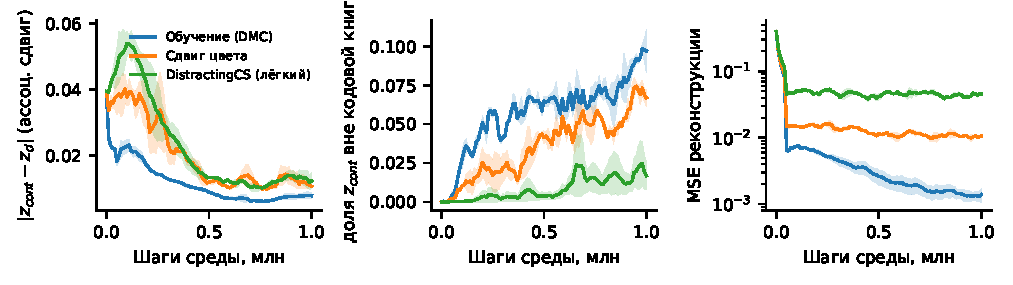
\includegraphics[width=\textwidth]{figures/latent_stats_ru}}
\caption{Латентные статистики на оценочных кадрах в ходе обучения (среднее по
2 сидам, заливка~--- разброс между сидами). Слева: средний ассоциативный сдвиг
$|z_{cont}-z_d|$. В центре: доля выходов энкодера за пределами диапазона их
кодовой книги. Справа: MSE реконструкции $g_\phi(z_d)$ относительно
наблюдаемого (возможно, с помехами) кадра, логарифмическая шкала.}
\label{fig:latent}
\end{center}
\vskip -0.2in
\end{figure*}

Главное утверждение ALDA: латентная модель переводит OOD-латенты к значениям
из обучающего распределения. Мы проверяем две вещи: (а)~заметно ли больше
ассоциативная поправка на OOD-кадрах? (б)~связана ли её величина с потерей
награды?

\paragraph{(а) На OOD-кадрах ассоциация срабатывает сильнее.} После первых
$2{\cdot}10^5$ шагов средний сдвиг $|z_{cont}-z_d|$ в среднем в $1,73$ раза
больше на кадрах со сдвигом цвета и в $1,80$ раза больше на кадрах DCS, чем на
обучающих (рис.~\ref{fig:latent}, слева). В начале обучения, пока энкодер ещё
не привязался к кодовой книге, сдвиг велик во всех трёх средах, и на OOD он
примерно в 2--3 раза больше, чем на обучающей. При этом OOD-кодировки
\emph{не} выходят за диапазон кодовой книги чаще (рис.~\ref{fig:latent}, в
центре). На обучающих кадрах около 9--10\% выходов энкодера лежат за крайними
значениями кодовой книги (энкодер проскакивает их, и ассоциация обрезает
значение), а на DCS~--- лишь 1--3\%. Значит, OOD-входы попадают \emph{между}
запомненными значениями, где мягкое извлечение Хопфилда с $\beta{=}100$ должно
выбрать одного из двух соседей и может выбрать не того. Ошибка реконструкции
относительно кадра с помехами (рис.~\ref{fig:latent}, справа) в 10 раз (цвет)
и в 30 раз (DCS) выше, чем на обучающей среде, и не меняется в ходе обучения.
Это согласуется с тем, что помеха отбрасывается, а не восстанавливается
(рис.~\ref{fig:recon}).

\begin{figure*}[t]
\vskip 0.1in
\begin{center}
\centerline{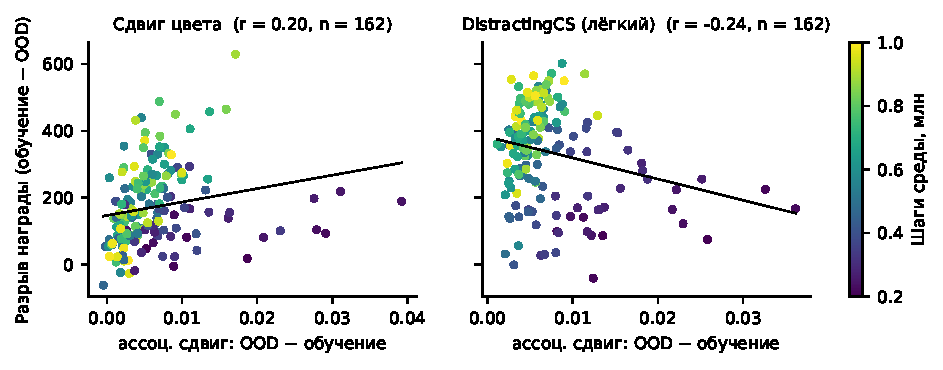
\includegraphics[width=0.85\textwidth]{figures/rq_scatter_ru}}
\caption{Ассоциативный сдвиг (OOD минус обучающая среда) и разрыв в награде
(обучающая минус OOD) для каждой оценки, оба сида, оценки после $2{\cdot}10^5$
шагов. Цвет показывает прогресс обучения; линия~--- подгонка методом
наименьших квадратов.}
\label{fig:rq}
\end{center}
\vskip -0.2in
\end{figure*}

\paragraph{(б) Величина поправки не предсказывает потерю.} По всем оценкам
после $2{\cdot}10^5$ шагов (81 на сид, $n{=}162$) корреляция Пирсона между
разностью ассоциативных сдвигов (OOD минус обучающая) и разрывом в награде
(обучающая минус OOD) равна $0,20$ для сдвига цвета и $-0,24$ для DCS. Обе
корреляции слабые и разного знака. За время обучения сдвиг \emph{уменьшается}
(рис.~\ref{fig:latent}, слева), а разрыв в награде в абсолютных значениях
\emph{растёт} (рис.~\ref{fig:returns}). Средняя величина ассоциации плохо
показывает, помогает ли она. Рис.~\ref{fig:rq} показывает, что слабая
корреляция объясняется прогрессом обучения: у ранних оценок (тёмные точки)
сдвиг большой, а разрыв маленький, потому что награда пока низкая везде.
Среди поздних, светлых точек тренда не видно.

\paragraph{Ответ.} Да, на OOD-наблюдениях ассоциативная латентная модель
срабатывает сильнее. Качественно она делает то, что заявлено в ALDA: внешний
вид помех переводится к виду обучающей среды. Но то, насколько сильно она
сдвигает латенты, не предсказывает качество. Мы предполагаем, что качество
зависит от того, сохраняют ли извлечённые значения важные для задачи факторы
(позу): провалы в DCS на рис.~\ref{fig:recon}~--- это ошибки позы, а фон в
реконструкцию не просачивается. Более точная диагностика измеряла бы ошибки
извлечения в латентах, которые кодируют важные для задачи факторы, но для
этого нужны истинные состояния среды для оценочных кадров. Это мы оставляем
на будущее.

\section{Ограничения и открытые вопросы}
\label{sec:limits}

\begin{itemize}
\item \textbf{Охват.} До 1~млн шагов обучен только walker-walk с 2 сидами.
  Конфигурации для cartpole-balance, ball\_in\_cup-catch и finger-spin есть и
  проходят короткие тестовые запуски, но полностью не обучались. В статье
  5 сидов и 4 задачи.
\item \textbf{Нет базовых методов.} Мы не обучали SAC+AE, SVEA и вариант
  SAC+QLAE с тем же бюджетом, поэтому не можем приписать OOD-награду именно
  ассоциации. Самый информативный следующий эксперимент~--- абляция,
  заменяющая уравнение~(\ref{eq:assoc}) жёстким квантованием.
\item \textbf{Среды.} Наш сдвиг цвета~--- это цветовое возмущение из DCS, а
  не среда «color hard» из DMCGB; DCS оценивается только на уровне easy.
\item \textbf{Неоднозначности.} В таблице статьи указан Adam; мы используем
  AdamW для энкодера и декодера (раздел~\ref{sec:impl}). Точная маршрутизация
  градиентов и архитектура энкодера истории восстановлены по рис.~2 статьи и
  могут отличаться от кода авторов.
\end{itemize}

\section{Заключение}

Наша однофайловая реализация SAC+ALDA учится решать walker-walk по пикселям
и без всякой аугментации переносится без дообучения на незнакомые сдвиги
цвета (81\% награды на обучающей среде) и частично на Distracting Control
Suite (43\%). Обе OOD-кривые продолжают расти по ходу обучения. Реконструкции
показывают, что ассоциативная латентная модель переводит наблюдения с
помехами к виду обучающей среды. Однако средняя величина её поправки не
объясняет оставшийся разрыв в качестве; по-видимому, он вызван ошибками в
позе агента при сдвиге камеры.

\section*{Код и данные}

Код, конфигурации и скрипты для графиков доступны по адресу
\url{https://github.com/zxclwnq/test-alda}. Обучение:
\texttt{python alda.py configs/walker\_walk.yaml seed=1}. Графики:
\texttt{python report/plots.py ru} и \texttt{python report/plots\_extra.py ru}
(без аргумента \texttt{ru}~--- с английскими подписями).

\section*{Влияние работы}

Цель этой работы~--- развитие области машинного обучения. У неё много
возможных общественных последствий, но ни одно из них, на наш взгляд, не
требует отдельного обсуждения.

\bibliography{example_paper}
\bibliographystyle{icml2025}

%%%%%%%%%%%%%%%%%%%%%%%%%%%%%%%%%%%%%%%%%%%%%%%%%%%%%%%%%%%%%%%%%%%%%%%%%%%%%%%
% APPENDIX
%%%%%%%%%%%%%%%%%%%%%%%%%%%%%%%%%%%%%%%%%%%%%%%%%%%%%%%%%%%%%%%%%%%%%%%%%%%%%%%
\newpage
\appendix
\onecolumn
\section{Визуализации для сида 2}

\begin{figure}[h]
\begin{center}
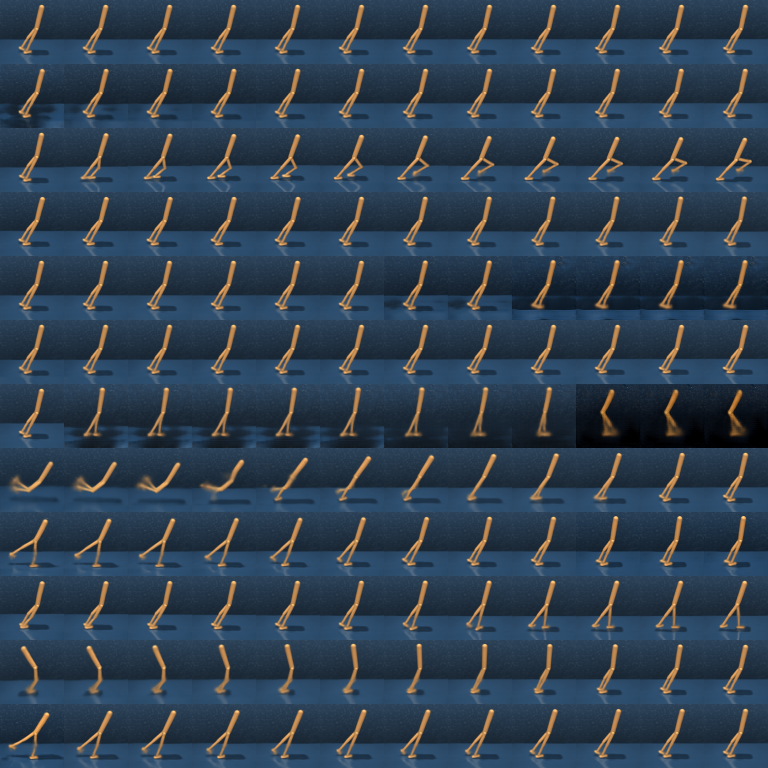
\includegraphics[width=0.48\textwidth]{figures/traversal_s2}
\hfill
\begin{minipage}[b]{0.48\textwidth}
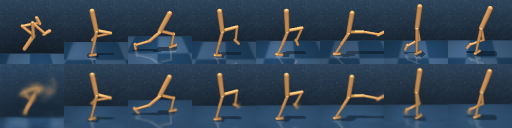
\includegraphics[width=\textwidth]{figures/recon_train_s2}\\[2pt]
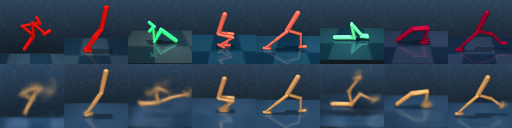
\includegraphics[width=\textwidth]{figures/recon_color_s2}\\[2pt]
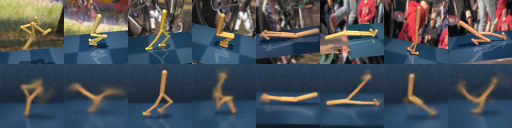
\includegraphics[width=\textwidth]{figures/recon_dcs_s2}
\end{minipage}
\caption{Сид 2 после 1~млн шагов. Слева: обход латентных переменных (как на
рис.~\ref{fig:traversal}). Справа: реконструкции на обучающей среде, при
сдвиге цвета и в Distracting CS (как на рис.~\ref{fig:recon}).}
\end{center}
\end{figure}

\section{Динамика обучения}

\begin{figure}[h]
\begin{center}
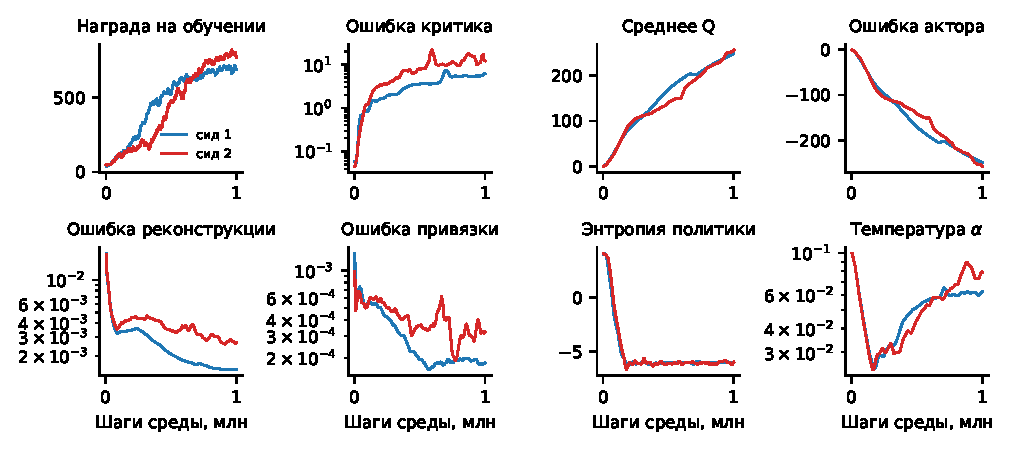
\includegraphics[width=\textwidth]{figures/training_dynamics_ru}
\caption{Статистики обучения по эпизодам (потери усреднены по обновлениям
внутри эпизода, скользящее среднее по 20 эпизодам). Энтропия стратегии
достигает целевого значения SAC $-|\mathcal{A}|=-6$ примерно за $10^5$ шагов,
после чего $\alpha$ подстраивается, чтобы удерживать её. У сида 2 ошибка
критика примерно вдвое выше, ошибки реконструкции и привязки тоже выше, но
и награда у него выше.}
\label{fig:dynamics}
\end{center}
\end{figure}

Ошибки реконструкции и привязки падают на порядок за первые $5{\cdot}10^4$
шагов и затем продолжают медленно уменьшаться (рис.~\ref{fig:dynamics}).
Ошибка привязки остаётся на два порядка ниже ошибки реконструкции, то есть
энкодер держится близко к кодовой книге без явного $\mathcal{L}_{quantize}$.
Среднее $Q$ растёт плавно, ошибка критика не расходится.

\section{Эволюция реконструкций и обходов латентов}

\begin{figure}[h]
\begin{center}
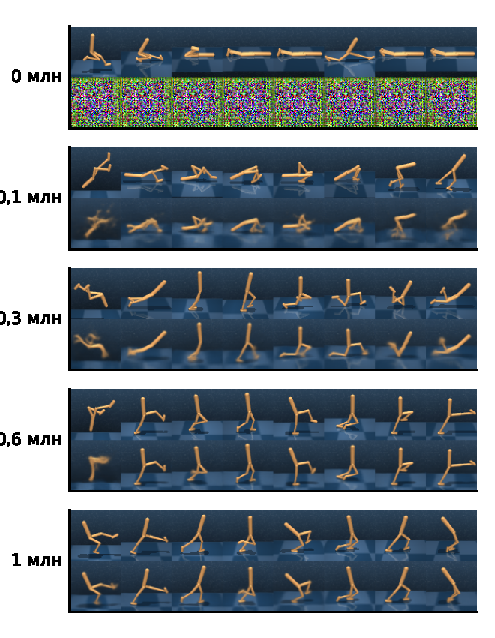
\includegraphics[width=0.32\textwidth]{figures/recon_train_evolution_ru}
\hfill
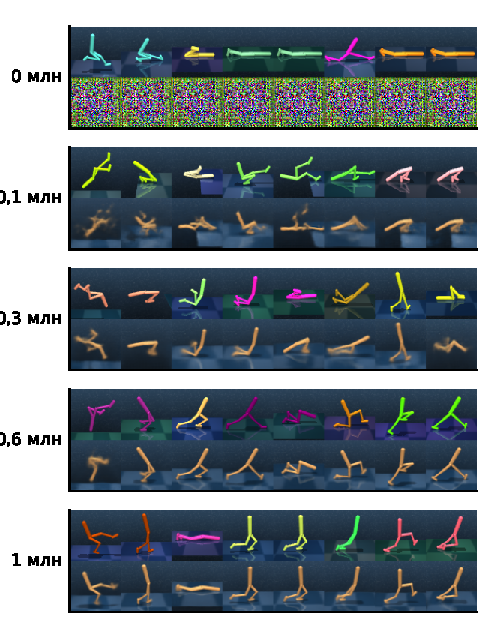
\includegraphics[width=0.32\textwidth]{figures/recon_color_evolution_ru}
\hfill
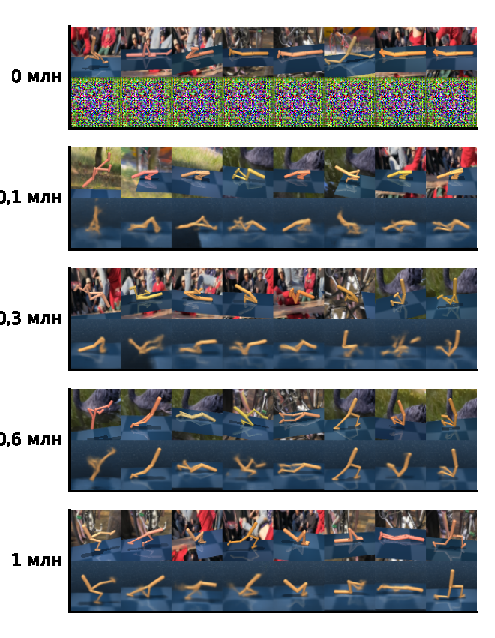
\includegraphics[width=0.32\textwidth]{figures/recon_dcs_evolution_ru}
\caption{Входы и реконструкции после 0; 0,1; 0,3; 0,6 и 1~млн шагов (сид 1,
из журнала изображений TensorBoard). Слева направо: обучающая среда, сдвиг
цвета, Distracting CS. Уже с 0,1~млн шагов фоны и цвета из OOD-сред
декодируются как обучающая сцена; дальше обучение в основном делает позу
агента чётче.}
\label{fig:recon-evo}
\end{center}
\end{figure}

\begin{figure}[h]
\begin{center}
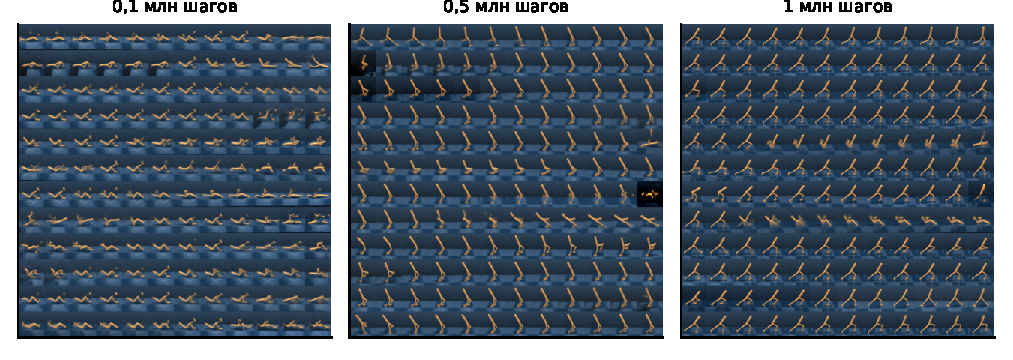
\includegraphics[width=\textwidth]{figures/traversal_evolution_ru}
\caption{Обход латентных переменных после 0,1; 0,5 и 1~млн шагов (сид 1). На
0,1~млн большинство латентов почти не меняет изображение; к 0,5~млн
несколько латентов управляют отдельными положениями конечностей и корпуса, а к
1~млн обходы становятся плавнее.}
\label{fig:trav-evo}
\end{center}
\end{figure}

\end{document}
